

 En este capítulo se comentará el proceso seguido para la realización de este proyecto detallando la planificación, diseño y el desarrollo de interfaces.
 
\section{Pasos de ejecución}

Una vez hecho el análisis, conocidos los objetivos que se quieren alcanzar en este proyecto y las herramientas que se utilizarán  empezaremos con la planificación del mismo.

Un punto muy  importante a tener en cuenta a la hora de realizar una planificación sería conocer los recursos y el tiempo del que disponemos.
Este punto tan crucial se acentúa ya que este proyecto será realizado por una única persona.

Para realizar la planificación del proyecto hemos dividido el proyecto en tareas con unos objetivos bien marcados(Product Backlog). A su vez al seguir la metodología Scrum dividimos el proyecto en etapas (Sprint) de tiempo donde incluimos las tareas a realizar.
 En todas estas etapas incluimos los siguientes pasos:
 
 


\begin{itemize}
\item Definición del Sprint Backlog,  documento que recoge las historias de usuario y quién las desempeña. En este caso al solo trabajar el estudiante en el proyecto haré todas las tareas.


\item División de las historias de del Sprint en tareas más sencillas y abordables. 



\item Diseño de cada una de las tareas del punto anterior.
\item  Implementacion de las tareas.
\item Pruebas.
\end{itemize}



\section{Duración  y costes}
 A continuación en la tabla \ref{fig:coste} se ha realizado una estimación de tiempos y de costes de este proyecto.
 Cuando se realiza una estimación de costes tenemos que tener en cuenta los gastos en material, licencias y los gastos propios. En mi caso los gastos de material y de licencias es nulo ya que el material es el del alumno y licencias y gastos propios son nulos.
 En la siguiente tabla se detalla el esfuerzo horas-hombre de cada uno de los roles dentro del proyecto. 
 
 La jornada laboral sería de 5 horas, 5 días a la semana y la duración de cada Sprint 4 semanas, lo que nos hace obtener el siguiente coste:


\begin{figure}[H]
		\centering
		\includegraphics[width=0.75\textwidth] {coste.png}
		\caption{Costes asociados a este proyecto }
		\label{fig:coste}
	\end{figure}






\begin{itemize}
\item En el rol de jefe de proyecto estaría a cargo de los que 
supervisan y evalúan el proyecto. En este caso los directores realizarán este rol.

\item Analista/programador Junior, en este rol estaría la persona encargada de las tareas de análisis, diseño, desarrollo y de la creación de las pruebas para este proyecto. Al estar realizado por el estudiante este se encargaría de este rol.





\end{itemize}
\section{Sprints}

Como se comentó a lo largo de este capítulo la metodología usada será  Scrum y el proyecto será dividido en Sprints de 4 semanas cada uno. El número de Sprint  estimados sería de 8.




 Antes de empezar con los Sprints comenzamos creando el Product Backlog. Esto es una lista con todas las funcionalidades del la aplicación priorizadas de más a menos importancia para nuestro proyecto. 

\subsection{Sprint 1}

En este primer Sprint nos centramos en las tareas relacionadas con la capa intermedia. Para ello comenzamos diseñando el modelo de datos, algo fundamental en cualquier aplicación para no heredar carencias en capas superiores, y acabamos implementando el modulo de servicios.


\subsection{Sprint 2}
 Una vez implementado el modulo servicio , el objetivo en este Sprint era hacer las pruebas para él.
 Una vez acabas las pruebas el siguiente paso dentro de este Sprint era la creación de las maquetas que sirvieron para la capa de presentación/cliente, es decir, el interfaz del usuario. Estas maquetas se fueron revisando y refinando a lo largo del proyecto.
 
\subsection{Sprint 3}

En este Sprint se comenzó con el desarrollo de la aplicación Android. Comenzamos permitiendo que el usuario fuera capaz que conocer su localización dentro del mapa y que al ir desplazándose cambie su ubicación como también obtener las coordenadas de su posición. Este punto será básico para el resto de la aplicación ya que nos proporciona los datos necesarios para guardar puntos y rutas. Las historias que se implementarán serán \textbf{creación de los puntos de interés (caza y pesca)},\textbf{ búsqueda de PDIs por tipo} y \textbf{borrado de PDIs} los casos de uso realizados son los siguientes:

\begin{itemize}

\item\textbf{\textit{ R-PDI-1 Guardar Punto De Interés caza}}  (vea Figura \ref{fig:pdicaza})
\item\textit{ \textbf{R-PDI-2 Guardar Punto De Interés pesca}}  (vea Figura \ref{fig:pdipesca})
\item \textbf{\textit{R-PDI-3 Eliminar PDI}}  (vea Figura \ref{fig:pdiborrar})
\item \textbf{\textit{R-PDI-4 Buscar los PDI}}  (vea Figura \ref{fig:pdiguardar})
\end{itemize} 


\begin{figure}[htbp]
\begin{minipage}[b]{0.5\linewidth} %Una minipágina que cubre la mitad de la página
\centering
\includegraphics[width=6cm]{capturamovil/pdipesca.png}
 
\caption{PDI pesca}
\label{fig:pdipesca}
\end{minipage}
\hspace{0.5cm} % Si queremos tener un poco de espacio entre las dos figuras
\begin{minipage}[b]{0.5\linewidth}
\centering
\includegraphics[width=6cm]{capturamovil/pdicaza.png}

\caption{PDI caza}
\label{fig:pdicaza}
\end{minipage}
\end{figure}



\begin{figure}[htbp]
\begin{minipage}[b]{0.5\linewidth} %Una minipágina que cubre la mitad de la página
\centering
\includegraphics[width=6cm]{capturamovil/pdiguardar.png}

\caption{Guardar PDI}
\label{fig:pdiguardar}
\end{minipage}
\hspace{0.5cm} % Si queremos tener un poco de espacio entre las dos figuras
\begin{minipage}[b]{0.5\linewidth}
\centering
\includegraphics[width=6cm]{capturamovil/pdiborrar.png}

\caption{Borrar PDI }
\label{fig:pdiborrar}
\end{minipage}
\end{figure}

En la pantalla tenemos los botones citados de arriba a abajo zoom sobre nosotros, eliminar PDI, cambiar el tipo de mapa y añadir PDI. 

\subsection{Sprint 4}

En este Sprint nos centraremos en las historias de  \textbf{Iniciar sesión }
\textbf{Registro} contiene los siguientes casos de uso:



\begin{itemize}
\item\textbf{ \textit{R1  Registrarse en la aplicación.}}  ( vea Figura \ref{fig:login})
\item \textbf{\textit{R2 Iniciar sesión en la aplicación. }}  (vea Figura \ref{fig:registro})

\end{itemize} 
\begin{figure}[htbp]
\begin{minipage}[b]{0.5\linewidth} %Una minipágina que cubre la mitad de la página
\centering
\includegraphics[width=6cm]{capturamovil/login.png}

\caption{Iniciar sesión }
\label{fig:login}
\end{minipage}
\hspace{0.5cm} % Si queremos tener un poco de espacio entre las dos figuras
\begin{minipage}[b]{0.5\linewidth}
\centering
\includegraphics[width=6cm]{capturamovil/registro.png}

\caption{Registro del usuario }
\label{fig:registro}
\end{minipage}
\end{figure}
Además en este Sprint hemos desarrollado un \textit{toolbar} para gestionar todas las opciones y mejorar la navegación del usuario en la aplicación.
\begin{figure}[H]
		\centering
		\includegraphics[width=0.5\textwidth] {capturamovil/opciones}
		\caption{Captura del menú de navegación}
	\end{figure}
\subsection{Sprint 5}
Este Sprint se centrará en las historias:

\begin{itemize}
\item \textbf{\textit{Creación de grupos}}, contiene los siguientes casos de uso:
\begin{itemize}
\item\textbf{ \textit{R-G-1 Crear grupo}} (vea  Figura~\ref{fig:creargrupo})
\item\textbf{\textit{ R-G-2 Añadir integrantes}}( vea Figura~\ref{fig:addintegrante})
\end{itemize}
\item \textbf{\textit{Eliminar grupos}}, que contiene el siguiente caso de uso:
\begin{itemize}
\item   \textbf{\textit{R-G-3 Eliminar integrantes}}
\end{itemize}
\item \textbf{\textit{Visualización de grupos}} ,  contiene los siguientes casos de uso:
\begin{itemize}
\item \textbf{\textit{R-G-4 Ver grupos}} (vea Figura~\ref{fig:vergrupos})

\item  \textbf{\textit{R-G-5 Ver integrantes grupo}} ( veaFigura~\ref{fig:verintegrantes})

\end{itemize}
\end{itemize}


 




\begin{figure}[htbp]
\begin{minipage}[b]{0.5\linewidth} %Una minipágina que cubre la mitad de la página
\centering
\includegraphics[width=6cm]{capturamovil/creargrupo.png}
\caption{Crear grupo}
 \label{fig:creargrupo}

\end{minipage}
\hspace{0.5cm} % Si queremos tener un poco de espacio entre las dos figuras
\begin{minipage}[b]{0.5\linewidth}
\centering
\includegraphics[width=6cm]{capturamovil/addintegrante.png}

\caption{Añadir usuarios a grupo }
 \label{fig:addintegrante}
\end{minipage}
\end{figure}


\begin{figure}[htbp]
\begin{minipage}[b]{0.5\linewidth} %Una minipágina que cubre la mitad de la página
\centering
\includegraphics[width=6cm]{capturamovil/vergrupos.png}
\caption{Ver grupos del usuario}
 \label{fig:vergrupos}

\end{minipage}
\hspace{0.5cm} % Si queremos tener un poco de espacio entre las dos figuras
\begin{minipage}[b]{0.5\linewidth}
\centering
\includegraphics[width=6cm]{capturamovil/verintegrantes.png}
\caption{Ver integrantes del grupo }
 \label{fig:verintegrantes}

\end{minipage}
\end{figure}
\newpage
\subsection{Sprint 6}
Este Sprint se centrará en \textbf{Iniciar una ruta individual}.

\begin{itemize}
\item Creación de la ruta, contiene los siguientes casos de uso:

\begin{itemize}
\item \textbf{\textit{R-R-1 Crear ruta}} (vea Figura~\ref{fig:crearruta})
\item \textbf{\textit{R-R-1.1 Iniciar ruta}}
\item\textbf{ \textit{R-R-1.2 Parar ruta}}
\item \textbf{\textit{R-R-1.3 Guardar ruta}} 
\end{itemize}
Figura~\ref{fig:individual-navegacion} uniendo los catos de uso R-R-1.1, R-R-1.2 y R-R-1.3. En la pantalla tenemos el botón para acercar el zoom a nuestra posición, cambiar el tipo de mapa y aumentar o disminuir el zoom. En la parte inferior derecha tenemos el botón para iniciar/para ruta y a la derecha de este finalizar ruta y salir de ella.
\item Ver las rutas seguidas por el usuario

\begin{itemize}
\item \textbf{\textit{R-R-3 Listar rutas} } (vea Figura \ref{fig:listarutas})

\end{itemize}
\item Ver una ruta en el mapa 

\begin{itemize}
\item \textbf{\textit{R-R-4 Ver ruta en mapa}}  (vea Figura \ref{fig:verruta})

\end{itemize}
\item Eliminar ruta

\begin{itemize}
\item \textbf{\textit{R-R-5 Eliminar ruta}} (vea Figura~\ref{fig:verruta1})

\end{itemize}

\end{itemize}








\begin{figure}[htbp]
\begin{minipage}[b]{0.5\linewidth} %Una minipágina que cubre la mitad de la página
\centering
\includegraphics[width=6cm]{capturamovil/crearruta.png}
\caption{Crear ruta}
 \label{fig:crearruta}

\end{minipage}
\hspace{0.5cm} % Si queremos tener un poco de espacio entre las dos figuras
\begin{minipage}[b]{0.5\linewidth}
\centering
\includegraphics[width=6cm]{capturamovil/individual-navegacion.png}
\caption{Navegación ruta individual }
 \label{fig:individual-navegacion}

\end{minipage}
\end{figure}


\begin{figure}[htbp]
\begin{minipage}[b]{0.5\linewidth} %Una minipágina que cubre la mitad de la página
\centering
\includegraphics[width=6cm]{capturamovil/verruta1.png}
\caption{Eliminar ruta}
 \label{fig:verruta1}

\end{minipage}
\hspace{0.5cm} % Si queremos tener un poco de espacio entre las dos figuras
\begin{minipage}[b]{0.5\linewidth}
\centering
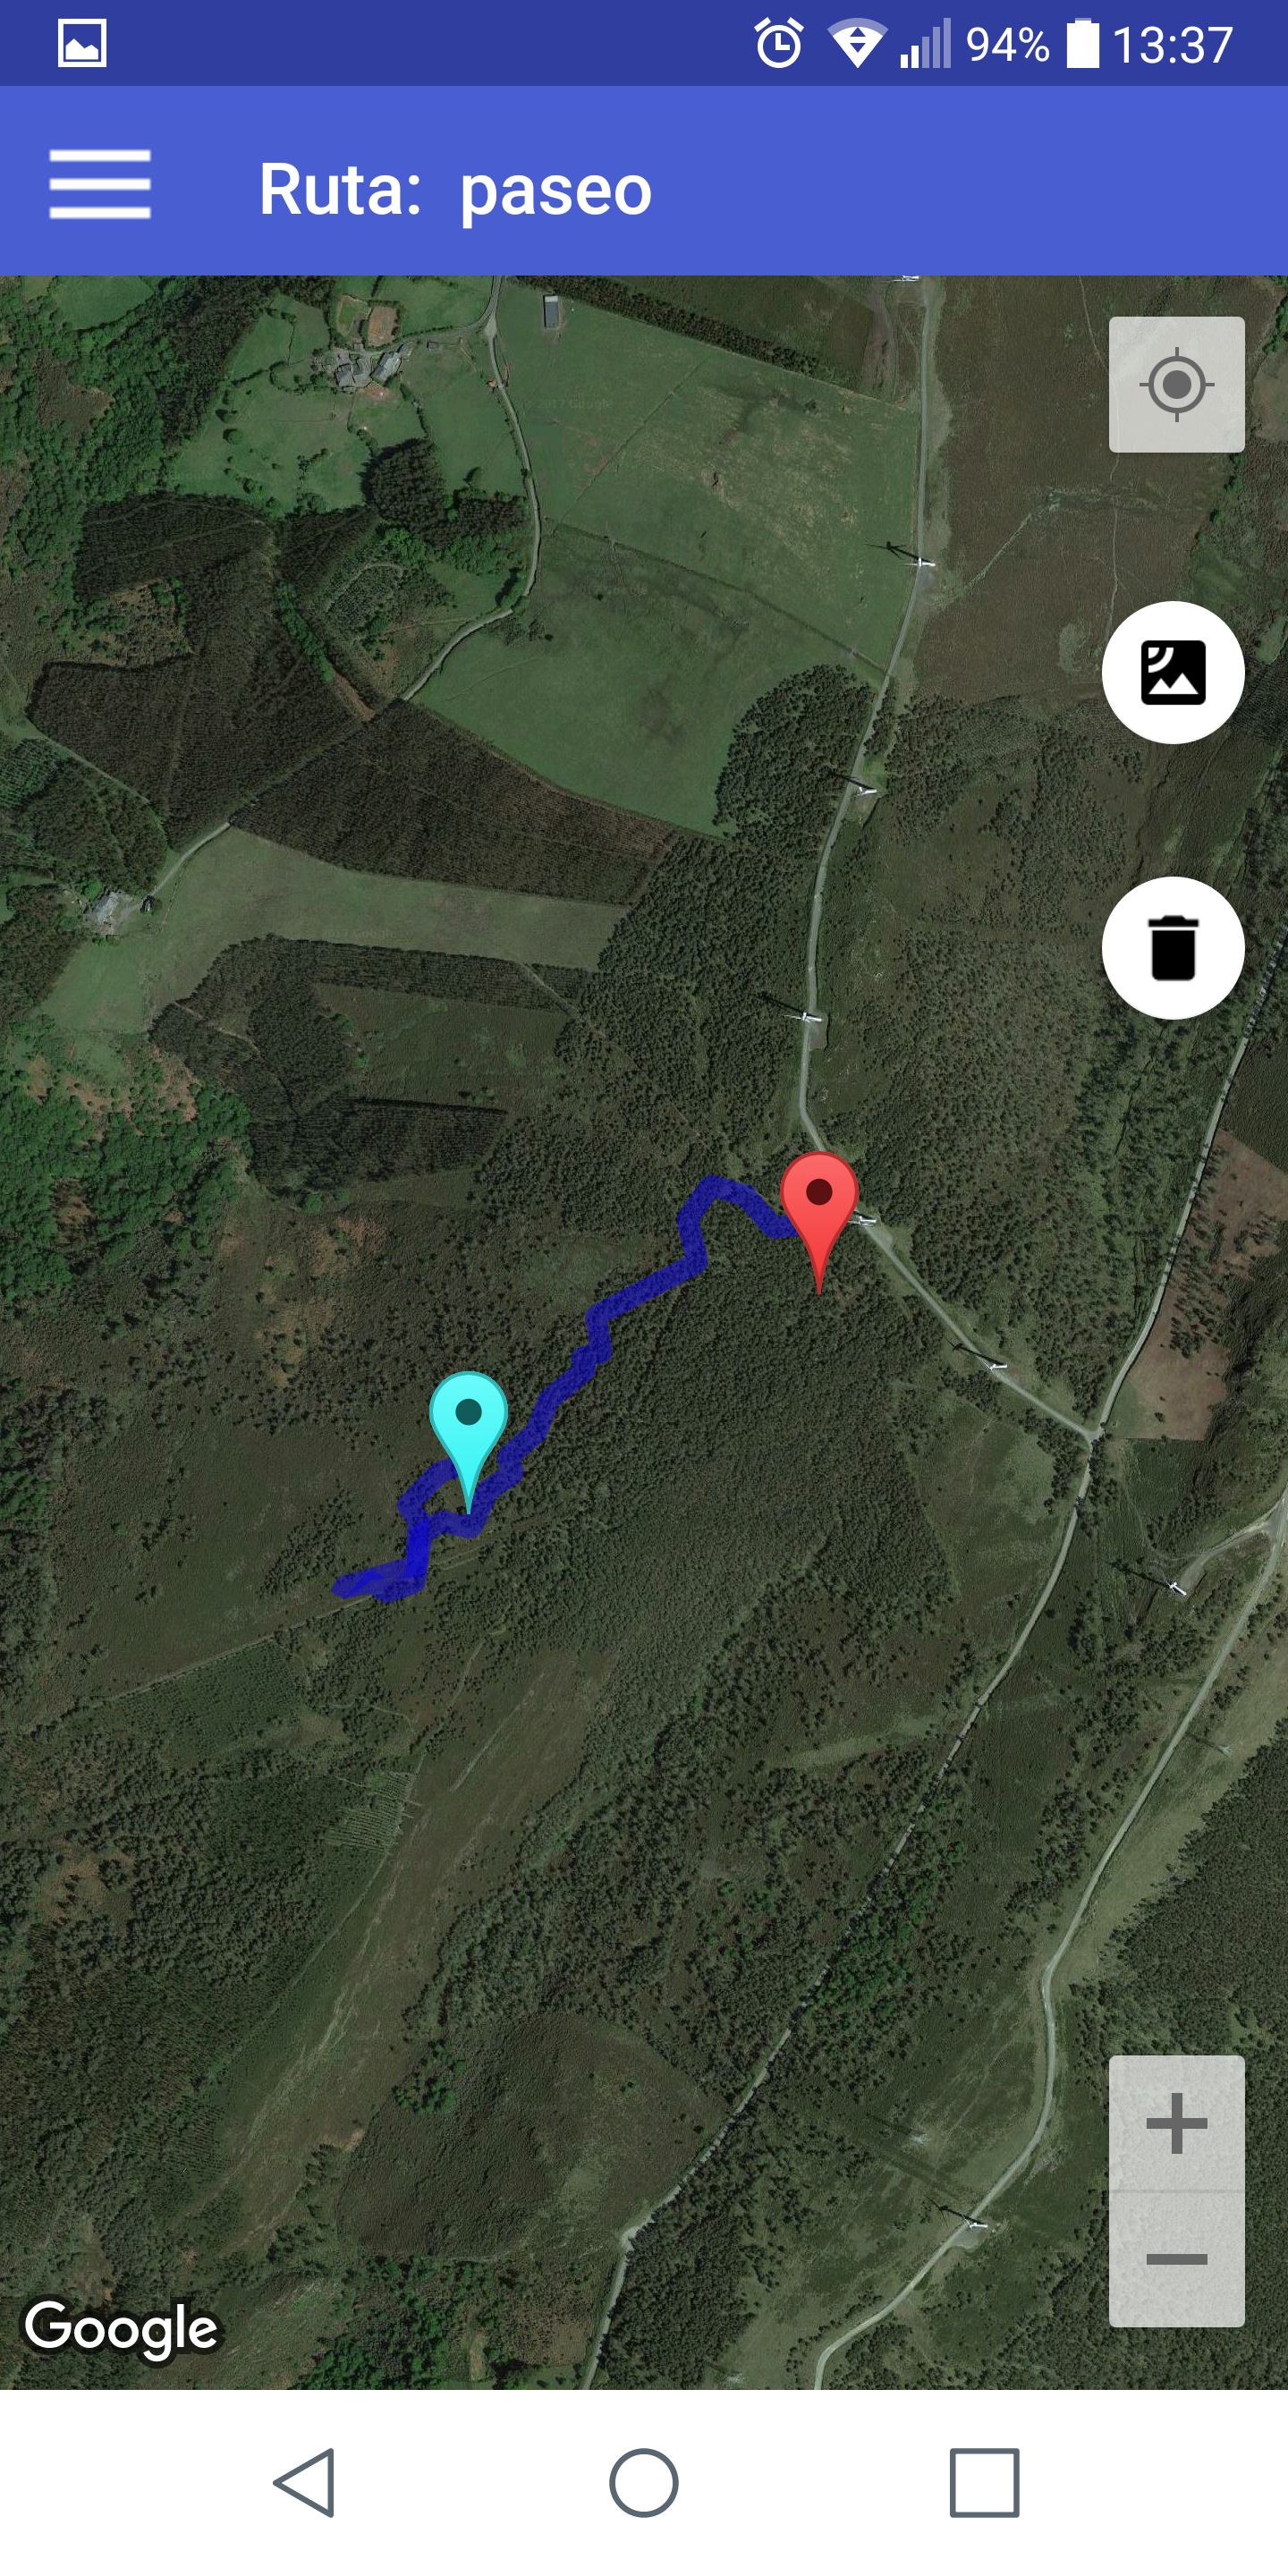
\includegraphics[width=6cm]{capturamovil/verruta2.png}
 
\caption{Ruta seguida vista satélite  }
\label{fig:verruta}
\end{minipage}
\end{figure}



\begin{figure}[htbp]
		\centering
		\includegraphics[width=0.5\textwidth] {capturamovil/listarutas}
		\caption{Lista de rutas creadas}
		 \label{fig:listarutas}
	\end{figure}
\newpage
\subsection{Sprint 7}
Este Sprint contiene la historia más compleja de todas,\textbf{ gestionar una ruta compartida},el interfaz es igual al de una ruta individual pero la lógica es diferente. (ver Figura~\ref{fig:individual-navegacion}).

\begin{itemize}
\item \textbf{\textit{R-R-2 Crear ruta compartida}}
\item \textbf{\textit{R-R-2.1 Iniciar ruta}}
\item \textbf{\textit{R-R-2.2 Parar ruta}}
\item \textbf{\textit{R-R-2.3 Finalizar ruta}}
\end{itemize}










\subsection{Sprint 8}

Por último en este Sprint se realizarán las pruebas finales, cierre del proyecto y la redacción de la memoria.

